\section{Two 4-transpositions}

\paragraph{}
If there are two 4-transpositions, there are 12 edges but the minimum number to link 11 points is 10. There are two "joker" edges. Thus there are three different possibilities for those "joker" edges: two double edges, one double edge and one alternating square or two alternating squares. We study this three cases.

\begin{lemma}
  If there are two double edges then they must be $(\rho_0, \rho_2)$ and $(\rho_1, \rho_3)$.
\end{lemma}

\begin{proof}
  If the difference between the indices of one alternating edge is not 2, this double must be adjacent to alternating square by Proposition~\ref{continue-double-edge}. But there are no alternating square, thus the difference of the indices must be 2. There are only two possibilities: $(\rho_0, \rho_2)$ and $(\rho_1, \rho_3)$

  \paragraph{}
  If there are two double edges $(\rho_0, \rho_2)$, then all $\rho_0$ edges have been used and the graph is the following.\footnote{Graph}

  \paragraph{}
  To connect the two $\rho_3$ edges, since no alternating square or double can be built, the $\rho_3$ edges must be surrounded by two $\rho_2$ edges (for more details see proof of Lemma~\ref{todo}). Furthermore a $\rho_3$ edge must use one of the two "ends" of the "chain".

  \paragraph{}
  Thus at least one double edge is not placed at one end of the graph and thus needs two $\rho_2$ edges to be connected. But the last double edge also needs at least one $\rho_2$ edge. And thus 5 $\rho_2$ edges are needed but that is impossible.

\end{proof}

\begin{lemma}
  If there are one double edge and one alternating square then they must be $(\rho_0, \rho_2)$ and $[\rho_1, \rho_3]$.
\end{lemma}

\begin{proof}
  If the indices of the double edge are consecutive, then this double edge must be adjacent to an alternating square. If the double edge is $(\rho_0, \rho_1)$, the alternating square must be $[\rho_0, \rho_2]$ but that does not make any sense\footnote{Why?}. If it is $(\rho_1, \rho_2)$, the alternating square can be $[\rho_0, \rho_2]$.\footnote{Graphs}.

  \paragraph{}
  None of the $\rho_3$ edges have been placed. Thus they need two $\rho_2$ edges. In both cases all $\rho_0$, $\rho_2$ and $\rho_3$ edges have been used and there are 3 remaining $\rho_1$ but it is impossible\footnote{Details}.

  \paragraph{}
  If the difference of the indices is 3, the double edge must be $(\rho_0, \rho_3)$ but the adjacent square must be $[\rho_1, \rho_3]$. There is a single $\rho_0$ edge remaining, this edge must be adjacent to a $\rho_1$ edge. There is only one $\rho_1$ edge for 4 $\rho_2$ edges, hence the graph can never be connected. Thus the index of the double edge must be separated by 2 and the double edge is $(\rho_0, \rho_2)$\footnote{Not complete}

  \paragraph{}
  No index 0 or 3 can be repeated in both patterns if they are distinct because the alternating square uses two edges. But $\rho_0$ and $\rho_3$ are 2-transpositions and thus have only two edges.

\end{proof}

\begin{lemma}
  If there are two alternating squares then they must be $[\rho_0, \rho_2]$ and $[\rho_1, \rho_3]$.
\end{lemma}

\begin{proof}
  The alternating square uses two edges. Thus no index $0$ or $3$ can be repeated.

  \paragraph{}
  If the index are consecutive, there must be an adjacent square by Lemma~\ref{continue-alternating-squaer}. There are two possibilities: $[\rho_0, \rho_1]$ or $[\rho_1, \rho_2]$. In the first case, there are no possible adjacent square. And in the second case, the only possibility is $[\rho_0, \rho_2]$. Furthermore, the $\rho_3$ edges need to be connected by two $\rho_2$ edges. But there are only one remaining.

  \paragraph{}
  If the square is $[\rho_0, \rho_3]$ then the adjacent square must be $[\rho_1, \rho_3]$. But the index $3$ is repeated and that is impossible.

  \paragraph{}
  Thus one alternating square must be $[\rho_0, \rho_2]$ and the other must be $[\rho_1, \rho_3]$.

\end{proof}

Now we list all the possible monodromy groups with rank 4 on $A_{11}$.

\begin{theorem}
  All monodromy groups of rank 4 on $A_{11}$ with two 4-transpositions are those presented in appendix~\ref{rank4-2-4transpositions} (p.~\pageref{rank4-2-4transpositions})).
\end{theorem}

\paragraph{}
The proof of this theorem is left to the reader because it is just a very simple (but long) application of the Method~\ref{method}.

\paragraph{}
There are a lot of monodromy groups, thus it is important to be systematic. The appendix~\ref{rank3-2-1-4-transposition} is structured in the following way and we encourage the reader to search for all monodromy groups in the same way.

\begin{enumerate}
  \item Choose which structures consume the "joker" edges: two double edges, one double edge and one alternating square or two alternating squares.
  \item Choose the length of the chain between the two structures.
  \item Choose the distance between one structure and the end of the graph.
\end{enumerate}

\paragraph{}
Once this decision tree is made, finding the graphs is very easy. The structure of appendix~\ref{rank4-2-4transpositions} matches the decision tree. It's important to check that the dual of the current graph has not already be found.

\paragraph{}
For each of this monodromy group we prove that it is not a string C-group representation of $A_{11}$. We make three sub-sections for the three main cases. The proofs are not complete. In the first examples a method is given to proof that the monodromy group is not a string C-group representation.

\subsection{Two double edges}

\begin{theorem}
  None of the monodromy groups with two double edges presented in appendix~\ref{rank4-2-1-4transpositions} are not string C-groups representation of $A_{11}$.
\end{theorem}

\begin{proof}
  For all the graphs we always consider $S_1 = \{\rho_1,\rho_2,\rho_3\}$ and $S_2 = \{\rho_2, \rho_3, \rho_4\}$. We must prove that $\Gamma_{S_1 \cap S_2} \neq \Gamma_{S_1} \cap \Gamma_{S_2}$.

  \paragraph{}
  We look at the first graph, the Figure~\ref{r4-1-1}. Here is one copy of this graph.

  \begin{figure}[H]
    \begin{center}
      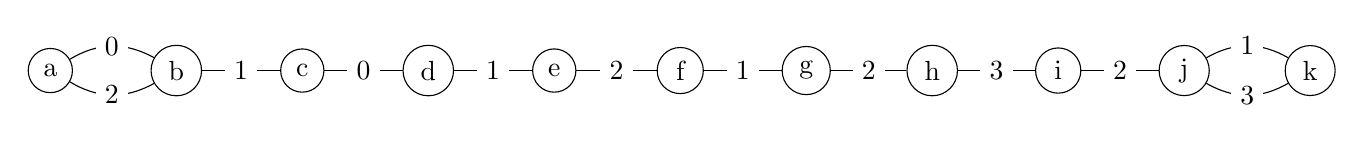
\begin{tikzpicture}[scale=.8]

        \begin{scope}[every node/.style={circle,draw}]
          \node (1)  at (0,0) {a};
          \node (2)  at (2,0) {b};
          \node (3)  at (4,0) {c};
          \node (4)  at (6,0)  {d};
          \node (5)  at (8,0)  {e};
          \node (6)  at (10,0)  {f};
          \node (7)  at (12,0)  {g};
          \node (8)  at (18,0)  {j};
          \node (9)  at (20,0)  {k};
          \node (10) at (16,0)  {i};
          \node (11) at (14,0)  {h};
        \end{scope}

        \begin{scope}[every node/.style={fill=white}]

          \begin{scope}[every edge/.style={draw}]
            \path (1)  edge[bend left=30] node {$0$} (2);
            \path (3)  edge node {$0$} (4);
            \path (2)  edge node {$1$} (3);
            \path (4)  edge node {$1$} (5);
            \path (6)  edge node {$1$} (7);
            \path (8)  edge[bend left=30] node {$1$} (9);
            \path (1)  edge[bend right=30] node {$2$} (2);
            \path (5)  edge node {$2$} (6);
            \path (7)  edge node {$2$} (11);
            \path (8)  edge node {$2$} (10);
            \path (8)  edge[bend right=30] node {$3$} (9);
            \path (10) edge node {$3$} (11);
          \end{scope}
        \end{scope}

      \end{tikzpicture}
      \caption{}
    \end{center}
  \end{figure}

  \paragraph{}
  Let's have a look at $\Gamma_{S_1}$ and $\Gamma_{S_2}$

  \begin{figure}[H]
    \begin{center}
      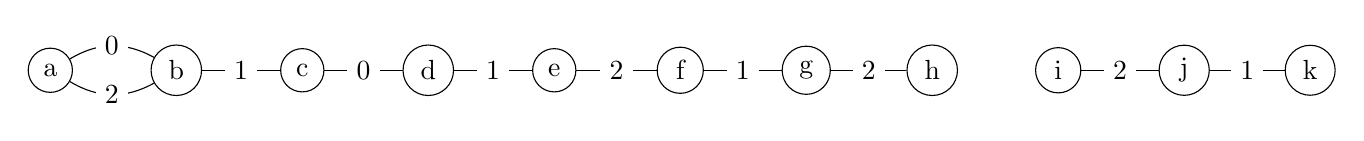
\begin{tikzpicture}[scale=.8]

        \begin{scope}[every node/.style={circle,draw}]
          \node (1)  at (0,0) {a};
          \node (2)  at (2,0) {b};
          \node (3)  at (4,0) {c};
          \node (4)  at (6,0)  {d};
          \node (5)  at (8,0)  {e};
          \node (6)  at (10,0)  {f};
          \node (7)  at (12,0)  {g};
          \node (8)  at (18,0)  {j};
          \node (9)  at (20,0)  {k};
          \node (10) at (16,0)  {i};
          \node (11) at (14,0)  {h};
        \end{scope}

        \begin{scope}[every node/.style={fill=white}]

          \begin{scope}[every edge/.style={draw}]
            \path (1)  edge[bend left=30] node {$0$} (2);
            \path (3)  edge node {$0$} (4);
            \path (2)  edge node {$1$} (3);
            \path (4)  edge node {$1$} (5);
            \path (6)  edge node {$1$} (7);
            \path (8)  edge node {$1$} (9);
            \path (1)  edge[bend right=30] node {$2$} (2);
            \path (5)  edge node {$2$} (6);
            \path (7)  edge node {$2$} (11);
            \path (8)  edge node {$2$} (10);
          \end{scope}
        \end{scope}

      \end{tikzpicture}
      \caption{$\Gamma_{S_1}$}
    \end{center}
  \end{figure}

  \begin{figure}[H]
    \begin{center}
      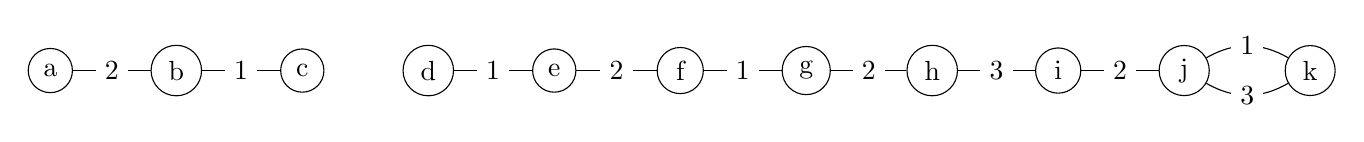
\begin{tikzpicture}[scale=.8]

        \begin{scope}[every node/.style={circle,draw}]
          \node (1)  at (0,0) {a};
          \node (2)  at (2,0) {b};
          \node (3)  at (4,0) {c};
          \node (4)  at (6,0)  {d};
          \node (5)  at (8,0)  {e};
          \node (6)  at (10,0)  {f};
          \node (7)  at (12,0)  {g};
          \node (8)  at (18,0)  {j};
          \node (9)  at (20,0)  {k};
          \node (10) at (16,0)  {i};
          \node (11) at (14,0)  {h};
        \end{scope}

        \begin{scope}[every node/.style={fill=white}]

          \begin{scope}[every edge/.style={draw}]
            \path (2)  edge node {$1$} (3);
            \path (4)  edge node {$1$} (5);
            \path (6)  edge node {$1$} (7);
            \path (8)  edge[bend left=30] node {$1$} (9);
            \path (1)  edge node {$2$} (2);
            \path (5)  edge node {$2$} (6);
            \path (7)  edge node {$2$} (11);
            \path (8)  edge node {$2$} (10);
            \path (8)  edge[bend right=30] node {$3$} (9);
            \path (10) edge node {$3$} (11);
          \end{scope}
        \end{scope}

      \end{tikzpicture}
      \caption{$\Gamma_{S_2}$}
    \end{center}
  \end{figure}

  \paragraph{}
  The group on the first graph is $A_8 : S_3$. This can be found by viewing that the component $\{a,b,c,d,e,f,g,h\}$ is $S_8$ and that there is a semi-direct product with the second component to keep parity. The second graph is also $A_8:S_3$.

  \paragraph{}
  The group $\Gamma_{S_1}$ can generate $S_5$ on the points $d,e,f,g,h$. Then points $a,b,c$ will be moved between them in order to the parity of the permutation even. This permutation is also in $\Gamma_{S_2}$, hence this group also generates $S_5$ on $d,e,f,g,h$. And the points $a,b,c$ are in $S_3$ and thus can always move to form the same permutation than in $\Gamma_{S_1}$.

  \paragraph{}
  Thus $\Gamma_{S_1} \cap \Gamma_{S_2} \ge S_5$ but $\Gamma_{S_1 \cap S_2} = \Gamma_{\rho_1, \rho_2} = D_{30}$. The order of $D_{30}$ is 30 and the order of $S_5$ is 120. Thus $\Gamma_{S_1} \cap \Gamma_{S_2} \neq \Gamma_{S_1 \cap S_2}$ and this monodromy group is not an string C-group representation of $A_{11}$.

  \paragraph{}
  The same kind of reasoning can be made for all graphs of Appendix~\ref{rank4-1-2-transpositions}. The results are displayed in Table~\ref{results-2-1}.

\begin{table}
  \centering
  \begin{tabular}{|c|c|c|c|c|c|c|}
    \hline
    Figure & $\Gamma_{S_1}$ & $\Gamma_{S_2}$ & $\Gamma_{S_1 \cap S_2}$ & $\#\Gamma_{S_1 \cap S_2}$ & $\Gamma_{S_1} \cap \Gamma_{S_2}$ & $\#(\Gamma_{S_1} \cap \Gamma_{S_2})$ \\ \hline

    \ref{r4-1-1} & $A_8 : S_3$ & $A_8 : S_3$ & $D_{30}$ & 30 & $\ge S_5$ & $\ge 120$ \\ \hline
    \ref{r4-1-2} & $A_5 \times 5 : 2$ & $A_8 : S_3$ & $D_{30}$ & 30 & & \\ \hline
    \ref{r4-1-3} & $A_7 \times 2 \times 2 : S_3$ & $A_7 \times 2 \times 2 : S_3$ & $D_{24}$ & 24 & & \\ \hline
    \ref{r4-1-4} & $S_7 \times 2 : 2$ & $A_7  \times 2 \cdot 2 : 2$ & $D_{24}$ & 24 & $\ge S_3$ & $\ge 6$ \\ \hline
    \ref{r4-1-5} & $A_8 : S_3$ & $A_5 \times 5 : 2$ & $D_{30}$ & 30 & & \\ \hline
    \ref{r4-1-6} & $A_8 : S_3$ & $A_{10}$ & $D_{42}$ & 42 & $\ge S_7$ & $\ge 5040$ \\ \hline
    \ref{r4-1-7} & $A_5 \times 5 : 2$ & $A_{10}$ & $D_{10}$ & 10 & & \\ \hline
    \ref{r4-1-8} & $A_{10}$ & $A_{10}$ & $D_{18}$ & 18 & $\ge A_9$ & $\ge 181400$ \\ \hline
    \ref{r4-1-9} & $A_{10}$ & $A_5 \times 5 : 2$ & $D_{10}$ & 10 & & \\ \hline
    \ref{r4-1-10}& $S_7 : D_8$ & $S_9$ & $D_{40}$ & 40 & $\ge S_6$ & $\ge 720$ \\ \hline
    \ref{r4-1-11}& $A_{10}$ & $A_5 : S_6$ & $D_{10}$ & 10 & $\ge S_5$ & $\ge 120$ \\ \hline
    \ref{r4-1-12}& $S_9$ & $A_7 \times 2 \times 2:S_3$ & $D_{40}$ & 40 & & \\ \hline
    \ref{r4-1-13}& $A_8 : S_3$ & $A_8 : S_3$ & $D_{30}$ & 30 & $\ge A_5$ & $\ge 60$ \\ \hline
    \ref{r4-1-14}& $A_8 : S_3$ & $A_{10}$ & $D_{42}$ & 42 & $\ge S_7$ & $\ge 5040$ \\ \hline
    \ref{r4-1-15}& $A_{10}$ & $A_{10}$ & $D_{18}$ & 18 & $\ge A_9$ & $\ge 181400$ \\ \hline
    \ref{r4-1-16}& $S_9$ & $S_9$ & $D_{28}$ & 28 & $\ge S_7$ & $\ge 5040$ \\ \hline
    \ref{r4-1-17}& $A_{10}$ & $A_8 : S_3$ & $D_{42}$ & 42 & $\ge S_7$ & $\ge 5040$ \\ \hline
    \ref{r4-1-18}& $A_{10}$ & $A_{10}$ & $D_{18}$ & 18 & $\ge A_9$ & $\ge 181440$ \\ \hline
    \ref{r4-1-19}& $A_{10}$ & $A_7 \times 2 \times 2 : S_3$ & $D_{42}$ & 42 & & \\ \hline
    \ref{r4-1-20}& $S_9$ & $A_5 : S_6$ & $D_{12}$ & 12 & $\ge S_4$ & $\ge 24$ \\ \hline
    \ref{r4-1-21}& $A_7 \times 2 \times 2 : S_{3}$ & $A_{10}$ & $D_{42}$ & 42 & & \\ \hline

  \end{tabular}
  \caption{}
  \label{results-2-1}
\end{table}

\subsection{One double edge and one alternating square}

\subsection{Two alternating squares}
  \paragraph{}
  This section can be done very easily by doing the same procedure that for the previous one. The results are displayed in Table~\ref{results-2-2}

  \begin{table}
    \centering
    \begin{tabular}{|c|c|c|c|c|c|c|}
      \hline
      Figure & $\Gamma_{S_1}$ & $\Gamma_{S_2}$ & $\Gamma_{S_1 \cap S_2}$ & $\#\Gamma_{S_1 \cap S_2}$ & $\Gamma_{S_1} \cap \Gamma_{S_2}$ & $\#(\Gamma_{S_1} \cap \Gamma_{S_2})$ \\ \hline

      \ref{r4-3-1} & $S_9$ & $S_9$ & $D_{28}$ & 28 & $\ge S_7$ & $\ge 5040$ \\ \hline
      \ref{r4-3-2} & $S_9$ & $A_8 : S_3$ & $D_{30}$ & 30 & $\ge S_6$ & $\ge 720$  \\ \hline
      \ref{r4-3-3} & $S_9$ & $S_9$ & $D_{28}$ & 28 & $\ge S_7$ & $\ge 5040$ \\ \hline
      \ref{r4-3-4} & $A_8 : S_3$ & $A_8 : S_3$ & $D_{30}$ & 30 & $\ge A_5$ & $\ge 60$ \\ \hline
      \ref{r4-3-5} & $A_8 : S_3$ & $A_8 : S_3$ & $D_{30}$ & 30 & $\ge A_5$ & $\ge 60$ \\ \hline
      \ref{r4-3-6} & $A_8 : S_3$ & $S_9$ & $D_{12}$ & 12 & $\ge S_6$ & $\ge 720$ \\ \hline
      \ref{r4-3-7} & $A_8 : S_3$ & $A_8 : S_3$ & $D_{30}$ & 30 & $\ge A_5$ & $\ge 60$  \\ \hline
      \ref{r4-3-8} & $S_7 \times D_8$ & $S_9$ & $D_{40}$ & 40 & $\ge S_5$ & $\ge 120$ \\ \hline
      \ref{r4-3-9} & $S_7 \times D_8$ & $S_9$ & $D_{40}$ & 40 & $\ge S_5$ & $\ge 120$ \\ \hline
      \ref{r4-3-10}& $S_9$ & $S_9$ & $D_{28}$ & 40 & $\ge S_7$ & $\ge 720$ \\ \hline

    \end{tabular}
    \caption{}
    \label{results-2-2}
  \end{table}

\end{proof}
